\section{Small sample inference for difference between two proportions}

%%%%%%%%%%%%%%%%%%%%%%%%%%%%%%%%%%%%

\begin{frame}
\frametitle{Comparing back of the hand to palm of the hand}

MythBusters also asked these people to guess the palms of their hands. This time 7 out of the 12 people guesses correctly. The data are summarized below.

\begin{center}
\begin{tabular}{ l | c | c | c }
          & Palm		& Back		& Total \\
\hline
Correct		& 11			& 7				& 18 \\
Wrong		  & 1				& 5				& 6 \\
\hline
Total			& 12			& 12			& 24 \\
\end{tabular}
\end{center}

\end{frame}

%%%%%%%%%%%%%%%%%%%%%%%%%%%%%%%%%%%%

\begin{frame}
\frametitle{Proportion of correct guesses}

{\small
\begin{center}
\begin{tabular}{ l | c | c | c }
          & Palm  	& Back		& Total \\
\hline
Correct		& 11			& 7				& 18 \\
Wrong		  & 1				& 5				& 6 \\
\hline
Total			& 12			& 12			& 24 \\
\end{tabular}
\end{center}

}

\begin{itemize}

\item Proportion of correct in the back group: $\frac{11}{12} = 0.916$

\item Proportion of correct in the palm group: $\frac{7}{12} = 0.583$

\item Difference: 33.3\% more correct in the back of the hand group.

\end{itemize}

\dq{Based on the proportions we calculated, do you think the chance of guessing the back of the hand correctly is different than palm of the hand?}

\end{frame}

%%%%%%%%%%%%%%%%%%%%%%%%%%%%%%%%%%%%

\begin{frame}
\frametitle{Hypotheses}

\dq{What are the hypotheses for comparing if the proportion of people who can guess the backs of their hands correctly is different than the proportion of people who can guess the palm of their hands correctly?}

\begin{itemize}
\item[$H_0$:] $p_{back} = p_{palm}$
\item[$H_0$:] $p_{back} \ne p_{palm}$
\end{itemize}

\end{frame}

%%%%%%%%%%%%%%%%%%%%%%%%%%%%%%%%%%%%

\begin{frame}
\frametitle{Conditions?}

\begin{itemize}

\item Independence - within groups, between groups?
\begin{itemize}
\item Within each group we can assume that the guess of one subject is independent of another.
\item Between groups independence is not satisfied - we have the same people guessing. However we'll assume they're independent guesses to continue with the analysis.
\end{itemize}

\item Sample size?
\begin{itemize}
\item $\hat{p}_{pool} = \frac{11 + 7}{12 + 12} = \frac{18}{24} = 0.75$
\item Expected successes in back group: $12 \times 0.75 = 9$, failures = 3
\item Expected successes in palm group: $12 \times 0.75 = 9$, failures = 3
\item Since S/F condition fails, we need to use simulation to compare the proportions.
\end{itemize}

\end{itemize}

\end{frame}

%%%%%%%%%%%%%%%%%%%%%%%%%%%%%%%%%%%%

\subsection{Randomization HT for comparing two proportions}

%%%%%%%%%%%%%%%%%%%%%%%%%%%%%%%%%%%%

\begin{frame}
\frametitle{Simulation scheme}

\begin{enumerate}

\item Use 24 index cards, where each card represents a subject.

\item Mark 18 of the cards as ``correct" and the remaining 6 as ``wrong".

\item Shuffle the cards and split into two groups of size 12, for back and palm.

\item Calculate the difference between the proportions of ``correct" in the back and palm decks, and record this number.

\item Repeat steps (3) and (4) many times to build a randomization distribution of differences in simulated proportions.

\end{enumerate}

\end{frame}

%%%%%%%%%%%%%%%%%%%%%%%%%%%%%%%%%%%%

\begin{frame}
\frametitle{Interpreting the simulation results}

When simulating the experiment under the assumption of independence, i.e. leaving things up to chance. \\

\vspace{0.5cm}

If results from the simulations based on the \hl{null model} look like the data, then we can determine that the difference between the proportions correct guesses in the two groups was simply \hl{due to chance}. \\

\vspace{0.5cm}

If the results from the simulations based on the null model do not look like the data, then we can determine that the difference between the proportions correct guesses in the two groups was not due to chance, but \hl{because people actually know the backs of their hands better}.

\end{frame}

%%%%%%%%%%%%%%%%%%%%%%%%%%%%%%%%%%%%

\begin{frame}
\frametitle{Simulation results}

\begin{itemize}

\item In the next slide you can see the result of a hypothesis test (using only 100 simulations to keep the results simple).

\item Each dot represents a difference in simulated proportion of successes. We can see that the distribution is centered at 0 (the null value).

\item We can also see that 9 out of the 100 simulations yielded simulated differences at least as large as the observed difference (p-value = 0.09).

\end{itemize}

\end{frame}

%%%%%%%%%%%%%%%%%%%%%%%%%%%%%%%%%%%%

\begin{frame}[fragile]
\frametitle{}

{\tiny
\begin{Verbatim}[frame=single, formatcom=\color{blue}]
hand = as.factor(c(rep("correct", 7), rep("wrong", 5), c(rep("correct", 11), rep("wrong", 1))))
gr = c(rep("palm",12),rep("back",12))
inference(hand, gr, est = "proportion", type = "ht", null = 0, alternative = "twosided",
	order = c("back","palm"), success = "correct", method = "simulation", seed = 879,
	nsim = 100)
\end{Verbatim}
}

\pause

{\tiny
\begin{Verbatim}[frame=single, formatcom=\color{gray}]
Response variable: categorical, Explanatory variable: categorical
Difference between two proportions -- success: correct
Summary statistics:
         x
y         back palm Sum
  correct   11    7  18
  wrong      1    5   6
  Sum       12   12  24
Observed difference between proportions (back-palm) = 0.3333
H0: p_back - p_palm = 0 
HA: p_back - p_palm != 0 
p-value =  0.18 
\end{Verbatim}
}

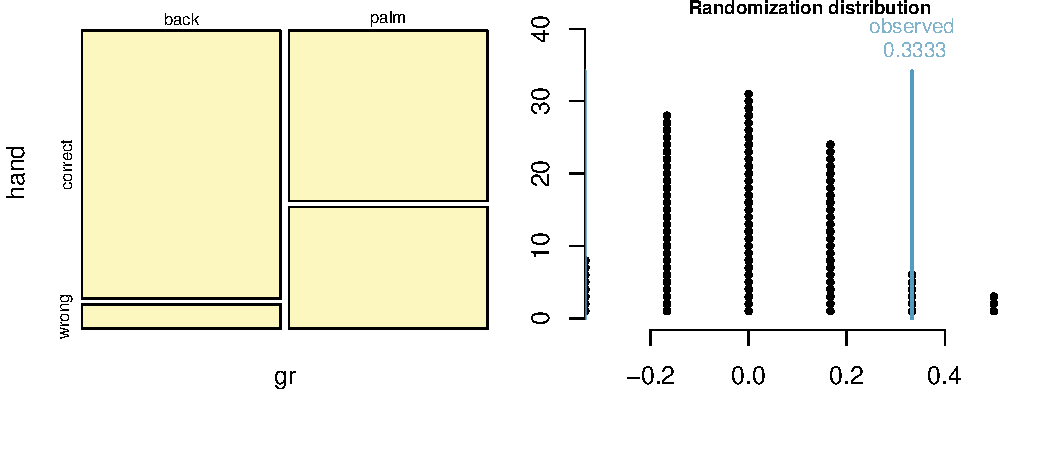
\includegraphics[width=0.8\textwidth,height=0.3\textheight]{6-6_small_two_props/figures/hand/palm_back_HT}

\end{frame}

%%%%%%%%%%%%%%%%%%%%%%%%%%%%%%%%%%%

\begin{frame}
\frametitle{Conclusion}

\pq{Do the simulation results suggest that people know the backs of their hands significantly better? \\
(Remember: There were 33.3\% more correct in the back group in the observed data.)}

\begin{enumerate}[(a)]
\item Yes
\solnMult{No}
\end{enumerate}

p-value = 0.09 $>$ 0.05, fail to reject $H_0$. The data do not provide convincing evidence that people know the backs of their hands better than the palms of their hands.

\end{frame}

%%%%%%%%%%%%%%%%%%%%%%%%%%%%%%%%%%%%%